\section{Grundlagen, Stand der Forschung}

\emph{Leseführung.} \lipsum[6-6]

% Und noch schnell die ganze Bibliographie zitieren:
\nocite{*}

\subsection{Theorie 1}

\emph{Informieren und orientieren.} Das Schema in Abbildung \ref{fig:software_struktur} enthält 
\lipsum[7-7]

\begin{figure}[H]
\begin{center}
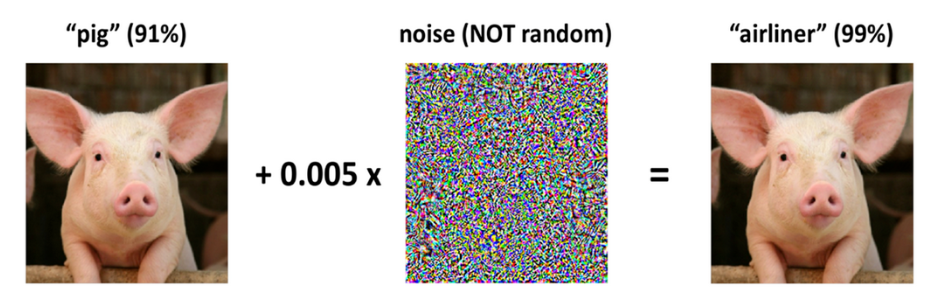
\includegraphics[width=\linewidth]{01-images/01-titleimage.png}
\end{center}
\caption{Realisierte Software-Struktur in LABView \\
\cite{engstrom_discussion_2019}}
\label{fig:software_struktur}
\end{figure}

\lipsum[1]

\subsection{Theorie 2}

\lipsum[8]  Nach Formel \eqref{eq:sincos}:
\begin{equation}[H]
\sin \alpha \pm \sin \beta = 2\sin\frac{\alpha\pm\beta}{2}\cos\frac{\alpha\mp\beta}{2}\,. \label{eq:sincos}
\end{equation}

\lipsum[9]
\begin{equation}[H]
x = \frac{-b\pm\sqrt{b^2-4ac}}{2a}\;.
\end{equation}

\lipsum[9-10]
